%
%  Created by Adam Ladachowski on 2012-03-31.
%
\documentclass[9pt,a4paper,twocolumn]{extarticle}

\usepackage{extsizes}

% \usepackage{polski}

\usepackage[top=2cm,bottom=2cm,left=2cm,right=2cm]{geometry}
\usepackage{fancyhdr}
\pagestyle{fancy}

%\usepackage{fontspec}
\usepackage{xunicode}
\usepackage{xltxtra}
\usepackage[none]{hyphenat}

% Set Sans as the default font
\renewcommand{\familydefault}{\sfdefault}
\renewcommand{\headrulewidth}{0pt}

% Lets see how a star will look like as item list bullet
\renewcommand{\labelitemi}{$\star$}

\setlength{\parindent}{0pt} 
\setlength{\parskip}{0cm}
\setlength{\columnsep}{2cm}


\fancyhead[L]{{\bf email:} adam.ladachowski@gmail.com, {\bf mobile:} +48 535 329 895, {\bf blog:} http://aladac.tumblr.com, {\bf twitter:} @aladac}
\fancyfoot{}
\fancyfoot[L]{\tt\small I hereby agree for my personal data, included in my job application, to be processed in line with the needs of 
recruitment, in accordance with the Personnel Protection Act of 29.08.1997 no 133 position 883}

\title{CV}
\author{Adam Ladachowski}

\begin{document}
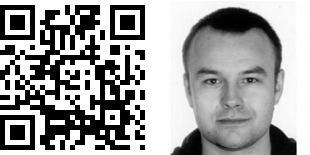
\includegraphics[width=\columnwidth]{photo_qr.png}
\vspace{0.2cm}

\section*{Adam Ladachowski}
born 1979, Warsaw resident

\section*{Objective}

Acquiring a stable, interesting and challenging job in IT or telecommunications

\section*{Availability}

3 months notice period, preferred place of employment: Warsaw, Poland

\section*{Profile}

System engineering, high level programming, design and development of utility and service software, acquiring new technology knowledge, team leadership, project management

\section*{Technical Skills}

\subsection*{Operating Systems}
Linux, Unix, Mac OS X, Windows
\subsection*{Programming}
Ruby, Ruby on Rails, Shell, AWK, SQL, PHP, Perl, C
\subsection*{SCM}
Git, Subversion
\subsection*{Text Markup}
DocBook, \LaTeX, HTML, HAML
\subsection*{Networking}
TCP/IP, Ethernet, ISDN DSS1, SMPP, UCP EMI
\subsection*{Services}
Apache, Kannel, Asterisk, SSH, SMTP, IMAP, POP
\subsection*{Databases}
MySQL, SQLite, PostgreSQL, MongoDB

\section*{Other Skills}
\subsection*{Languages}
native Polish, fluent English
\subsection*{Drivers License}
Category B, 1997

\section*{Certifications and Courses}

First Certificate in English (Cambridge, 1995)\\
Central Backup Management (BigVent, 2002)\\
CCNA Workshop Sessions (Altkom, 2004)\\
Advanced Driving (ABJ, 2006)\\
Artproject – Project Management (ArtED, 2007)\\
IP Telephony – SIP (CITCOM PW, 2007)\\
ISDN (CITCOM-PW, 2007)\\
Mobile Data Gateway (Materna, 2007)\\
Dedicated F5 Training (Compendium, 2009)\\

\section*{Experience}

{\bf Support and Development Team Coordinator}\\
at Materna Communications\\
(April 2006 – Present)
\begin{itemize}
\setlength{\itemsep}{0cm}%
\setlength{\parskip}{0cm}%
\item key account support and project coordination
\item project management
\item active role in recruitment
\item software development (Ruby, Ruby on Rails)
\item technical support of the sales process
\item system engineering (Linux, mobile messaging)
\item technical coordinator of fixed 
\item network SMSC project
\item developer of CDR rating platform for MVNE
\item project manager of MVNO provisioning platform development 
\end{itemize}

{\bf Service Support Specialist}\\
at Materna Communications \\
(April 2003 – April 2006) \\
second level support of SMS based managed services, software development (PHP, Perl), Solaris and Linux system administration \\

{\bf Computer System Administrator }\\
at Rema 1000 Poland G.A.Ladachowscy \\
(July 2002 – April 2003) \\
administration of stores computer system and network \\

{\bf Hosting Specialist }\\
at TDC Internet Polska \\
(December 2001 – July 2002) \\
second level support, management of ISP services run on Linux, Apache, qmail \\

{\bf Support Specialist }\\
at Polska OnLine \\
(January 2000 – December 2001) \\
first line support, DSL installations, Linux server installations\\

{\bf Unix System Administrator }
at Polnet Technologies International \\
(February 1999 – July 1999) \\
administration of a Large fault tolerant Unix and Oracle based system used in banking \\

{\bf\Large Hobbies and Interests}\\

mobile devices, Anime, computer and video games, sci-fi, comic books, rollerblades, paintball, laser tag\\

http://www.engadget.com/\\
http://www.goldenline.pl/\\
http://www.xda-developers.com/\\
http://stackoverflow.com/\\
http://kotaku.com/\\

\end{document}
